\documentclass[10pt]{article}

\input{/Users/gabesekeres/Dropbox/LaTeX_Docs/pset_preamble.tex}

\course{ECON 6110}
\pset{5}
\begin{document}
\maketitle


\subsection*{Problem 1}

The game can be written as:

\begin{figure}[H]
	\centering
	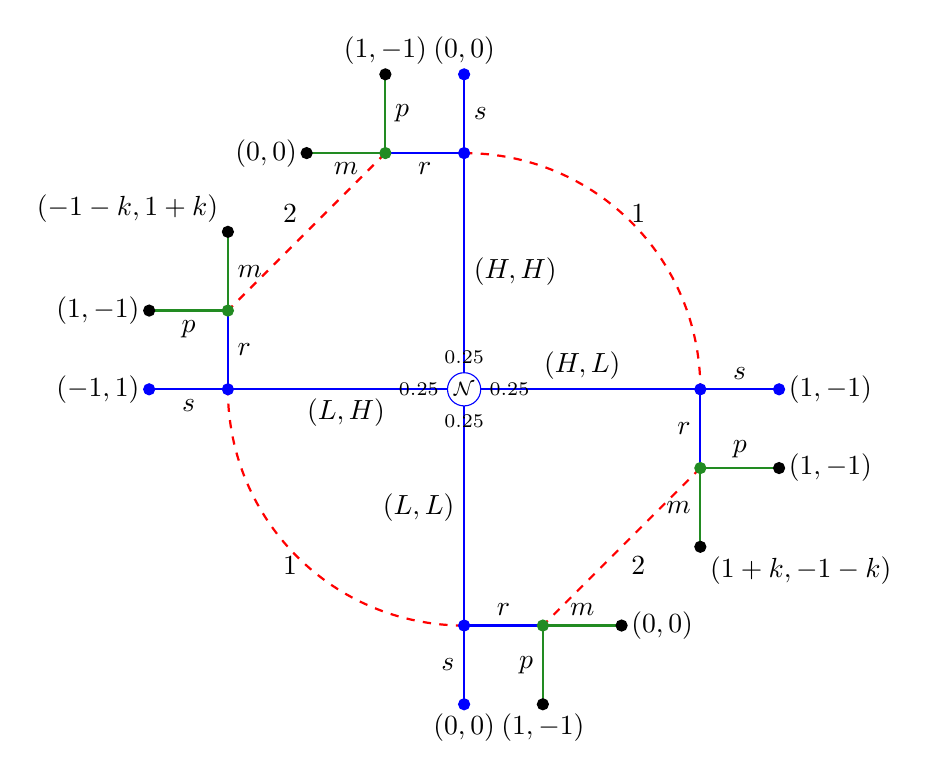
\begin{tikzpicture}
		
		
		\draw[blue,thick] (0,3)--(0,-3);
		\draw[blue,thick] (3,0)--(-3,0);
		\draw[blue,thick] (0,4)--(0,3)--(-1,3);
		\draw[blue,thick] (4,0)--(3,0)--(3,-1);
		\draw[blue,thick] (-4,0)--(-3,0)--(-3,1);
		\draw[blue,thick] (0,-4)--(0,-3)--(1,-3);
		\draw[ForestGreen,thick] (-2,3)--(-1,3)--(-1,4);
		\draw[ForestGreen,thick] (-3,2)--(-3,1)--(-4,1);
		\draw[ForestGreen,thick] (2,-3)--(1,-3)--(1,-4);
		\draw[ForestGreen,thick] (3,-2)--(3,-1)--(4,-1);
		
		\draw[red,dashed,thick] (0,3) to[out=0,in=90] (3,0);
		\draw[red,dashed,thick] (0,-3) to[out=180,in=-90] (-3,0);
		\draw[red,dashed,thick] (3,-1)--(1,-3);
		\draw[red,dashed,thick] (-1,3)--(-3,1);
		\node[above] at (1.5,0) {$(H,L)$};
		\node[right] at (0,1.5) {$(H,H)$};
		\node[left] at (0,-1.5) {$(L,L)$};
		\node[below] at (-1.5,0) {$(L,H)$};
		\node[right] at (0.2,0) {\scriptsize $0.25$};
		\node[left] at (-0.2,0) {\scriptsize $0.25$};
		\node[above] at (0,0.2) {\scriptsize $0.25$};
		\node[below] at (0,-0.2) {\scriptsize $0.25$};
		\node[below left] at (-2,-2) {$\bm{1}$};
		\node[above right] at (2,2) {$\bm{1}$};
		\node[above left] at (-2,2) {$\bm{2}$};
		\node[below right] at (2,-2) {$\bm{2}$};
		\node[right] at (0,3.5) {$s$};
		\node[left] at (0,-3.5) {$s$};
		\node[above] at (3.5,0) {$s$};
		\node[below] at (-3.5,0) {$s$};
		\node[below] at (-0.5,3) {$r$};
		\node[left] at (3,-0.5) {$r$};
		\node[above] at (0.5,-3) {$r$};
		\node[right] at (-3,0.5) {$r$};
		\node[right] at (-1,3.5) {$p$};
		\node[below] at (-3.5,1) {$p$};
		\node[above] at (3.5,-1) {$p$};
		\node[left] at (1,-3.5) {$p$};
		\node[below] at (-1.5,3) {$m$};
		\node[right] at (-3,1.5) {$m$};
		\node[left] at (3,-1.5) {$m$};
		\node[above] at (1.5,-3) {$m$};
		
		
		\filldraw[blue] (0,3) circle(2pt);
		\filldraw[blue] (0,-3) circle(2pt);
		\filldraw[blue] (3,0) circle(2pt);
		\filldraw[blue] (-3,0) circle(2pt);
		\filldraw[blue] (0,4) circle(2pt);
		\filldraw[blue] (0,-4) circle(2pt);
		\filldraw[ForestGreen] (1,-3) circle(2pt);
		\filldraw[ForestGreen] (-1,3) circle(2pt);
		\filldraw[blue] (4,0) circle(2pt);
		\filldraw[blue] (-4,0) circle(2pt);
		\filldraw[ForestGreen] (3,-1) circle(2pt);
		\filldraw[ForestGreen] (-3,1) circle(2pt);
		\filldraw[black] (3,-2) circle(2pt);
		\filldraw[black] (4,-1) circle(2pt);
		\filldraw[black] (2,-3) circle(2pt);
		\filldraw[black] (1,-4) circle(2pt);
		\filldraw[black] (-2,3) circle(2pt);
		\filldraw[black] (-1,4) circle(2pt);
		\filldraw[black] (-3,2) circle(2pt);
		\filldraw[black] (-4,1) circle(2pt);
		\filldraw[blue,fill=white] (0,0) circle(6pt);
		\node at (0,0) {\scriptsize$\bm{\mathcal{N}}$};
		
		
		\node[above] at (0,4) {$(0,0)$};
		\node[below] at (0,-4) {$(0,0)$};
		\node[right] at (4,0) {$(1,-1)$};
		\node[left] at (-4,0) {$(-1,1)$};
		\node[above] at (-1,4) {$(1,-1)$};
		\node[below] at (1,-4) {$(1,-1)$};
		\node[right] at (4,-1) {$(1,-1)$};
		\node[left] at (-4,1) {$(1,-1)$};
		\node[left] at (-2,3) {$(0,0)$};
		\node[right] at (2,-3) {$(0,0)$};
		\node[above left] at (-3,2) {$(-1-k,1+k)$};
		\node[below right] at (3,-2) {$(1+k,-1-k)$};
	\end{tikzpicture}
\end{figure}

Nature chooses the types, with (implied) probability of $0.25$ for each. Player 1 only knows her own card, and can not tell what player 2's card is. She chooses see ($s$) or raise ($r$) after viewing her card. If she chooses see, players compare and the game ends. If she chooses raise, player 2 has the chance to pass ($p$) or meet ($m$), after which the game ends. Player 2 knows only whether player 1 has chosen to raise and her card. In the extensive game, the dashed lines represent information sets, and the number on them is the player who moves in that information set. For readability, Player 1's nodes and the lines to and from them are in \textcolor{blue}{blue}, Player 2's nodes and the lines from them are in \textcolor{ForestGreen}{green}, information sets are in \textcolor{red}{red}, and outcome nodes are in black. Actions, types, probabilities, outcomes, and nature are all in black text because making you read colored text would be immoral. 




\newpage
\subsection*{Problem 2}

Define $\mu$ as the belief player 2 has that player 1 has played $M$, given that they are called to act. Observe that $U_1(L) > U_1(R)$ if and only if $\mu > \frac{1}{2}$, and similar with other inequalities. Thus, if Player 1 chooses such that $\mu > \frac{1}{2}$, then player 2 will always play $L$. In that case, player 1 strictly prefers $M$, so they will always play $M$, and $\mu = 1$. This is a pure strategy PBE, where $\sigma_1 = M$, $\sigma_2 = L$, and $\mu_2(M) = 1$. Note that the beliefs are derived from Bayes' Rule, as they are always attained on-path.

Observe also that if $\mu < \frac{1}{2}$, player 2 will always choose $R$, so player 1 will prefer $L$ to either $M$ or $R$ (weakly). Thus, we have another pure strategy PBE, where $\sigma_1 = L$, $\sigma_2 = R$, and beliefs are any $\mu_2(M) \in \barl 0,\frac{1}{2}\parr$. Since these beliefs are reached off-path, they are not subject to Bayes' Rule, so we can impose them exogenously.

Finally, we consider the case where $\mu = \frac{1}{2}$. Assume that player 2 chooses $L$ with probability $p \in [0,1]$. Player 1 is indifferent, so any mix will maximize their expected payoff. Player 1 will prefer $L$ as long as \begin{align*} 3p - 2(1-p) \le 1 &\Longrightarrow p \le \frac{3}{5} \\ 2p - (1-p) \le 1 &\Longrightarrow p \le \frac{2}{3}\end{align*}The tighter bound is $\frac{3}{5}$, so we'll hold that. If $p > \frac{3}{5}$, then player 2 would deviate to $M$ all the time, which would violate the assumption that $\mu = \frac{1}{2}$. Thus, we say that $p \le \frac{3}{5}$. Then player 1 will choose $L$ all the time, and since $M/R$ are off-path we can exogenously impose the correct beliefs. Thus, there is a third equilibrium in which $\sigma_1 = L$, $\sigma_2 =p \cdot L + (1-p)\cdot R$, for $p \in \barl 0,\frac{3}{5}\barr $, and $\mu_2(M) = \frac{1}{2}$. 

Thus, our PBE are:
\begin{align*}
	\sigma = (M, L),&\quad \mu = 1 \\\sigma = (L,R),&\quad \mu \in \barl 0 ,\frac{1}{2}\parr \\ \sigma = (L,p\cdot L + (1-p)\cdot R),&\quad \mu = \frac{1}{2}
\end{align*}



\subsection*{Problem 3}

\begin{itemize}
	\item[(a)] Assume that Player 2 believes $a_1$ is uninformative. Then they clearly maximize by always choosing $a_2 = -\frac{1}{2}$. Knowing that Player 2 believes $a_1$ is uninformative, Player 1 does not improve by sending any signal, so we'll say that they always send $a_1 = -1$. Then $u_1(-1) \ge u_1(a') = -\parl \frac{1}{2}-x_c\parr^2$, so $a_1=-1$ is (weakly) optimal given beliefs. Since $a_1 = -1 \forall w$, it is uninformative, so $\mu(w \mid a_1) = \mu(w) = \expect[w] = \frac{1}{2}$, so $a_2 = -\frac{1}{2}$ is optimal. This is a PBE since beliefs are rational and actions are optimal given beliefs.
	\item[(b)] Let's assume that $a_1 = -1$ when $w \in [0,w\opt]$ and $a_1=0$ when $w \in (w\opt,1]$. When Player 2 sees $a_1 = -1$, they will believe that $w \in [0,w\opt]$, so $\expect[w \mid a_1=-1] = \frac{w\opt}{2}$, and they attain their highest expected payoff by choosing $a_2 = -\frac{w\opt}{2}$, and when they see $a_1 = 0$ they will believe that $w \in (w\opt,1]$, so $\expect[w \mid a_1 = 0] = \frac{1+w\opt}{2}$, so they attain their highest expected payoff by choosing $a_2 = -\frac{1+w\opt}{2}$. We can impose exogenously that if they see $a_1 \not\in\{-1,0\}$ that they will view that signal as uninformative, and will choose $a_2 = -\frac{1}{2}$ as in part (a). Now go back to Player 1. They see $w \in [0,1]$, and knowing what Player 2 will do, they must have that \[u_1(-1: w \le w\opt) = -\parl w - \frac{w\opt}{2}-x_c\parr^2 \ge -\parl w - \frac{w\opt}{2}-x_c-\frac{1}{2}\parr^2 = u_1(0: w \le w\opt)\]and \[u_1(0: w > w\opt) = -\parl w - \frac{w\opt}{2}-x_c - \frac{1}{2}\parr^2 \ge -\parl w - \frac{w\opt}{2}-x_c\parr^2 = u_1(1:w>w\opt)\]These conditions hold if and only if they both hold at the boundary $w\opt$. We can solve the equation:\[-\parl \frac{w\opt}{2} - x_c\parr^2 = -\parl \frac{w\opt}{2} - x_c - \frac{1}{2}\parr^2  \Longrightarrow \frac{w\opt}{2} - x_c = \frac{1}{4} \Longrightarrow w\opt = \frac{1}{2} + 2x_c\]So as long as $x_c \le \frac{1}{4}$, setting $w\opt = \frac{1}{2}+2x_c$ maintains incentive compatibility, and this is an informative PBE.
\end{itemize}















\end{document}